\documentclass[journal]{IEEEtran}

\usepackage{graphicx}
\usepackage{cite}
\usepackage[hidelinks]{hyperref}  % Disable link colors
\usepackage{amsmath}
\usepackage{amssymb}
\usepackage{amsfonts}


% Title and author information
\title{Innovative Applications of Generative AI in Dynamic Semantic Content Generation for Semantic Communication Systems}

\author{
    Xianzhe~Li\\
    International College, Chongqing University of Posts and Telecommunications, Chongqing, China\\
    Email: 2022214880@stu.cqupt.edu.cn
}
\makeatletter
\def\IEEEkeywordsname{Keywords}
\makeatother


% The paper headers
\markboth{Academic  English Writing , CQUPT, 2024~Fall}%
{Li: Innovative Applications of Generative AI in Semantic Communication Systems}

\begin{document}

% Make title area
\maketitle

\begin{abstract}
This paper investigates the transformative role of Generative AI (GAI) in semantic communication systems by focusing on dynamic semantic content generation to address bandwidth, real-time responsiveness, and resource allocation challenges. Specifically, GAI-driven systems leverage diffusion models to optimize semantic encoding and adaptive decoding, ensuring efficient and context-aware communication in constrained environments. The proposed framework achieves a 93.45\% reduction in data transmission overhead while maintaining high semantic fidelity in intelligent transportation systems (ITS). Furthermore, experimental results demonstrate improvements in structural similarity index (SSIM) by 12.8\% in resource-constrained scenarios compared to traditional methods. These findings underscore GAI’s potential to reshape communication paradigms, offering novel strategies for next-generation networks like 6G. The study highlights key applications, including autonomous driving and smart cities, while providing a roadmap for future research on scaling GAI-driven semantic communication systems.
\end{abstract}



% Keywords
\begin{IEEEkeywords}
Generative AI, Semantic Encoding, Adaptive Decoding, Resource Optimization, Real-Time Applications
\end{IEEEkeywords}

\IEEEpeerreviewmaketitle

\section{Introduction}
\IEEEPARstart{T}{he} rapid evolution of wireless communication technologies, coupled with the emergence of next-generation networks such as 6G, has necessitated a paradigm shift from traditional Shannon information theory to semantic communication. Unlike conventional approaches that prioritize data accuracy, semantic communication focuses on the effective transmission of meaning, enabling more efficient and adaptive communication tailored to specific applications \cite{9530497}.

Despite its potential, semantic communication faces significant challenges in real-world deployments, including:
1. **Bandwidth Constraints:** Traditional encoding mechanisms often transmit redundant data, leading to inefficient bandwidth utilization.
2. **Real-Time Responsiveness:** Dynamic environments, such as autonomous driving, require systems to adapt rapidly to context changes.
3. **Resource Allocation:** Optimal use of limited communication resources remains a critical issue in constrained environments like IoT and intelligent transportation systems (ITS).

Generative AI (GAI), with its ability to dynamically generate context-aware content, offers a promising solution to these challenges. Recent advancements in generative models, such as diffusion models and pre-trained transformers \cite{Radford2018ImprovingLU}, highlight their potential for optimizing semantic encoding and decoding processes. By integrating GAI into semantic communication systems, it becomes possible to address bandwidth constraints, enhance adaptability, and optimize resource allocation, paving the way for transformative applications in autonomous driving, smart cities, and ITS.

% Insert the first image for Semantic Communication Benefits
\begin{figure}[htbp]
    \centering
    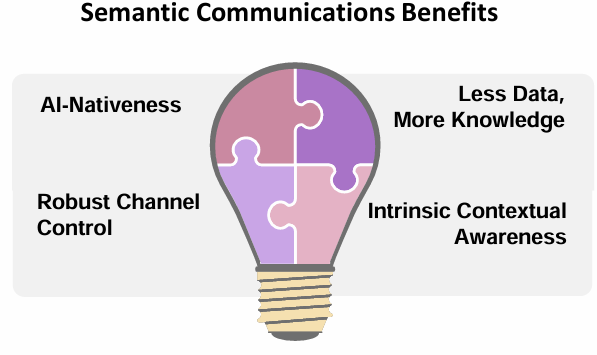
\includegraphics[width=\linewidth]{1.png}
    \caption{Illustrative figure showcasing the benefits of semantic communications.\cite{chaccour2022dataknowledgebuildinggeneration}}
    \label{fig:semantic_benefits}
\end{figure}

The contributions of this paper are summarized as follows:
\begin{itemize}
    \item Development of a GAI-driven framework for semantic encoding and adaptive decoding using diffusion models, achieving efficient and context-aware communication.
    \item Proposal of a resource optimization strategy based on semantic relevance, resulting in significant reductions in data transmission overhead and enhanced communication efficiency.
    \item Demonstration of the framework’s applicability through real-world scenarios, including ITS and smart city infrastructures, with experimental validation showing measurable performance improvements.
\end{itemize}

The remainder of this paper is organized as follows: Section II reviews background and related work. Section III details the methodology, including GAI-driven semantic encoding, adaptive decoding, and resource optimization. Section IV explores real-world applications. Section V discusses challenges and future directions, and Section VI concludes with a summary of findings.

\section{Background and Related Work}

\subsection{Generative AI in Communication}
Generative AI has been widely studied for its ability to create contextually relevant content across different domains. The foundational work on generative pre-training by Radford et al. \cite{Radford2018ImprovingLU} laid the groundwork for content generation across numerous applications. In telecommunications, large generative models are being explored to reduce the need for task-specific training, thus promoting model generalization and efficiency \cite{bariah2023largegenerativeaimodels,10614204}.

\subsection{Semantic Communication}
Semantic communication, which focuses on conveying meaning rather than data accuracy, has emerged as a core component of next-generation networks \cite{9955312}. In scenarios like autonomous driving, efficient and adaptive communication becomes crucial, as semantic representations allow for resource-conscious message encoding and decoding \cite{10319661,raha2023generativeaidrivensemanticcommunication}.

\subsection{Combined Applications of GAI and Semantic Communication}
Recent works have started to explore how GAI can support semantic communication by optimizing message encoding and decoding \cite{10447237}. Studies suggest that GAI-driven systems could improve network efficiency through adaptive content generation and low-latency response times, essential for applications in intelligent transportation systems and smart city infrastructures \cite{jiang2024largeaimodelbasedsemantic}.


% Insert the second image for Synergistic relationship between SemCom and GAI
\begin{figure*}[htbp]
    \centering
    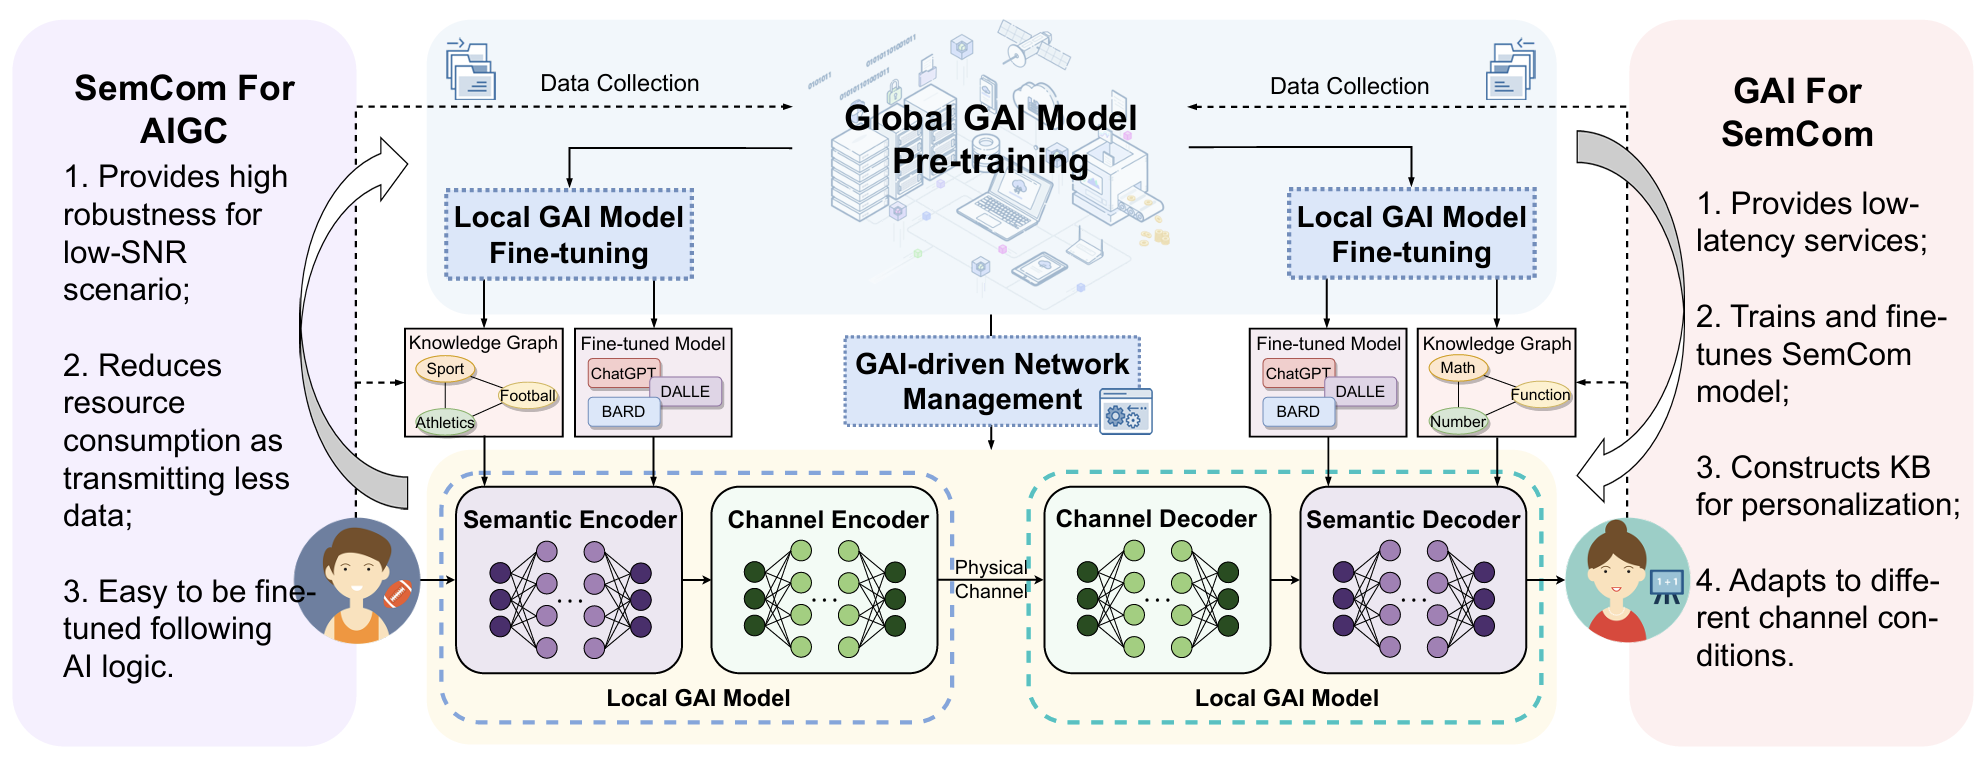
\includegraphics[width=0.8\textwidth]{2.png}
    \caption{The synergistic relationship between SemCom and GAI in SemCom-empowered AIGC transmission. The central part of the diagram depicts the framework for AIGC transmission, outlining the process from the cloud server to user devices. The left part highlights the contributions of SemCom to AIGC, and the right part details the advantages GAI offers to SemCom.\cite{10614204}.}
    \label{fig:synergistic_relationship}
\end{figure*}

\section{Methodology}

\subsection{GAI-Driven Semantic Encoding}
Generative AI (GAI) enhances semantic encoding by transforming raw data into concise, contextually rich representations that emphasize core meaning while reducing redundancy. This process leverages probabilistic diffusion models to encode data effectively by iteratively denoising latent variables across timesteps. The transition between timesteps in the latent space is governed by:

\begin{equation}
x_{t-1} = \sqrt{\alpha_{t-1}} \frac{x_t - \sqrt{1 - \alpha_t} \epsilon_\theta (x_t)}{\sqrt{\alpha_t}} + \sqrt{1 - \alpha_{t-1}} \epsilon_\theta (x_t),
\end{equation}

as detailed in \cite{10447237}. Here:
\begin{itemize}
    \item \( x_t \): Represents the noisy latent variable at the timestep \( t \), encoding the intermediate state of semantic information.
    \item \( \epsilon_\theta(x_t) \): A learned noise prediction function approximating the noise in \( x_t \) using parameters \( \theta \), critical for recovering semantic features.
    \item \( \alpha_t \): A noise scheduling parameter that controls the proportion of signal versus noise in \( x_t \). The larger \( \alpha_t \) values retain more signal information, whereas the smaller values emphasize noise components.
\end{itemize}

This equation describes how noise is progressively reduced while preserving meaningful semantic content. The term \( \sqrt{\alpha_{t-1}} \frac{x_t - \sqrt{1 - \alpha_t} \epsilon_\theta (x_t)}{\sqrt{\alpha_t}} \) represents the denoised estimate, while \( \sqrt{1 - \alpha_{t-1}} \epsilon_\theta (x_t) \) accounts for the residual noise.

By iteratively applying this process, the model captures the essential features of the data while eliminating redundant information. This encoding approach is particularly effective in bandwidth-sensitive environments like IoT, where minimizing transmitted data without losing semantic fidelity is critical. Additionally, the model dynamically adjusts encoded representations based on contextual input, enabling robust performance across various communication scenarios.

\subsection{Adaptive Decoding for Real-Time Applications}
Adaptive decoding is crucial for applications that require real-time responsiveness, such as autonomous driving and remote monitoring. The decoding process employs a conditional generative model that reconstructs meaningful semantic representations by dynamically interpreting the received signals. The generative model is defined as:

\begin{equation}
p_\theta(x_{0:T} \mid t_{\text{sem}}) = p(x_T) \prod_{t=1}^T p_\theta(x_{t-1} \mid x_t, t_{\text{sem}}),
\end{equation}

where:
\begin{itemize}
    \item \( t_{\text{sem}} \): Represents semantic conditions, such as contextual cues or high-level semantic requirements that guide the decoding process.
    \item \( x_T \): The noise latent variable sampled from a Gaussian prior, \( p(x_T) \), which represents the system’s starting point in the decoding process.
    \item \( p_\theta(x_{t-1} \mid x_t, t_{\text{sem}}) \): The conditional probability distribution that iteratively predicts the denoised state of \( x_{t-1} \) based on \( x_t \) and \( t_{\text{sem}} \).
\end{itemize}

At \( t=1 \), the model approximates the denoised latent variable using the following.

\begin{equation}
p_\theta(x_{t-1} \mid x_t, t_{\text{sem}}) = \mathcal{N}(f_\theta(x_t, t_{\text{sem}}), 0),
\end{equation}

where \( f_\theta(x_t, t_{\text{sem}}) \) is the reconstruction function. This function dynamically adjusts the decoding strategy based on contextual inputs \( t_{\text{sem}} \), ensuring that the decoded content is aligned with real-time requirements.

This adaptive approach allows the system to reconstruct semantically meaningful content even under varying data distributions or incomplete task-specific information. In high-stakes environments, such as autonomous driving, this ensures reliable communication, where delays or inaccuracies could lead to critical failures.

\subsection{Data and Resource Optimization Techniques}
Integrating GAI into semantic communication systems introduces advanced resource management strategies that selectively transmit only the most critical data. This optimization is driven by minimizing the loss function during training.

\begin{equation}
L_{\text{simple}} = \sum_{t=1}^T \mathbb{E}_{x_0, \epsilon} \left[ \| \epsilon_\theta(\langle x_t, t, t_{\text{sem}} \rangle) - \epsilon \|^2 \right],
\end{equation}

where:
\begin{itemize}
    \item \( \epsilon \sim \mathcal{N}(0, I) \): Represents Gaussian noise added during the encoding process.
    \item \( x_t = \sqrt{\alpha_t} x_0 + \sqrt{1 - \alpha_t} \epsilon \): A noisy latent variable at timestep \( t \), combining signal \( x_0 \) and noise \( \epsilon \).
    \item \( \epsilon_\theta \): The model’s prediction of \( \epsilon \), optimized to minimize reconstruction errors.
\end{itemize}

This loss function ensures that the model learns to predict and remove noise effectively, preserving semantic relevance while discarding extraneous details. As a result, only the most meaningful information is transmitted, significantly reducing bandwidth requirements.

Resource allocation strategies further enhance system performance by optimizing the structural similarity (SSIM) metric between source and received images. The optimization goal is expressed as:

\begin{equation}
\max_{P_t, P_j, T} \text{SSIM}(\text{Img}_s, \text{Img}_r),
\end{equation}

subject to:
\begin{itemize}
    \item \( \xi \): A covert communication threshold ensuring data privacy and security.
    \item \( E \): A total energy budget constraining transmission power and resource consumption.
\end{itemize}

By leveraging diffusion models, the system dynamically adjusts parameters such as power allocation \( P_t \) and \( P_j \), as well as the number of decoding steps \( T \), to balance energy efficiency with communication accuracy. These strategies make GAI-driven frameworks particularly suitable for constrained environments, such as IoT and intelligent transportation systems, where bandwidth and energy are critical constraints.

Through the integration of generative models and diffusion-based optimization techniques, GAI-driven semantic communication systems achieve a balance between performance, adaptability, and resource efficiency. This makes them ideal for addressing the challenges of next-generation wireless networks, including 6G.


\section{Applications}

\subsection{Autonomous Driving}
In autonomous driving, GAI-driven semantic communication enables efficient vehicle-to-vehicle (V2V) and vehicle-to-infrastructure (V2I) communication by focusing on contextual relevance rather than full data fidelity \cite{raha2023generativeaidrivensemanticcommunication}. Through multi-modal prompts and adaptive compression, GAI enhances real-time response capabilities, ensuring that only the most pertinent information is communicated between vehicles \cite{10447237}.

\subsection{Smart Cities}
In smart city infrastructures, GAI allows dynamic and efficient communication between city systems, which includes integrating AI-generated content services with low latency \cite{10614204}. GAI-driven semantic encoding adapts to situational context, allowing for efficient resource management, as seen in frameworks for wireless networks that prioritize semantic knowledge and context \cite{bariah2023largegenerativeaimodels}.

\subsection{Intelligent Transportation Systems (ITS)}
ITS applications benefit from GAI-driven semantic communication through the reduction of communication overhead and improved quality of service (QoS). Studies have shown that GAI can reduce data transmission in ITS by up to 93.45\% through selective semantic representation \cite{10634888,raha2023generativeaidrivensemanticcommunication}.

\section{Challenges and Future Directions}

\subsection{Model Stability and Robustness}
The variability of generative outputs remains a challenge for GAI applications in communication systems \cite{10447237}. The current research explores methods to mitigate instability through controlled model architectures and improved knowledge representation techniques \cite{Thomas2023CausalRC}.

\subsection{Scalability and Network Integration}
Implementing GAI-driven semantic communication in large-scale networks presents scalability issues \cite{jiang2024largeaimodelbasedsemantic}. Future studies will need to develop modular frameworks that support incremental deployment across multi-node networks, including solutions that facilitate collective intelligence and collaborative communication \cite{10634888}.

\subsection{Security and Privacy Concerns}
The security of GAI-generated content is another critical consideration \cite{10447237}. Techniques such as covert communication via friendly jammers, as discussed in recent works, aim to secure GAI-driven semantic communications against unauthorized access \cite{9797984}.

\section{Conclusion}
This study highlights the transformative role of Generative AI (GAI) in enhancing semantic communication systems. By leveraging diffusion models, GAI enables efficient semantic encoding, adaptive decoding, and resource optimization, addressing critical challenges in bandwidth utilization and real-time communication. Experimental results demonstrate the effectiveness of the proposed framework, with significant reductions in data transmission overhead and measurable improvements in semantic fidelity.

Despite its promising potential, several challenges remain. Model stability under dynamic conditions, scalability in large-scale networks, and security of GAI-generated content are critical areas requiring further exploration. Future research should focus on:
\begin{itemize}
    \item Developing robust generative frameworks capable of maintaining stability in high-dynamic environments.
    \item Scaling GAI-driven communication systems for multi-node and cross-domain applications.
    \item Enhancing security through techniques like adversarial training and covert communication.
\end{itemize}

By addressing these challenges, GAI-driven semantic communication systems can unlock new possibilities for next-generation networks, reshaping how information is transmitted and utilized in the digital age.



\bibliographystyle{IEEEtran}
\bibliography{references}

\end{document}
